\section{Uvod}

Tema ovog projekta je razvijanje globalnog informacionog sistema za Medj{}ugradski autobuski prevoz u nasoj zemlji. Rad je radj{}en kao projekat iz predmeta "Informacioni sistemi" na Matemati\v ckom fakultetu. Informacioni sistem bi trebao da olak\v sa probleme pri kupovini i rezervaciji karata. Omogu\'cava nam da bez odlaska na samu stanicu izvr\v simo rezervaciju karte kao i rezervaciju mesta ili eventualnu reklamaciju. Zaposlenima na autobuskoj stanici pru\v za uvid u slobodan broj mesta i olak\v sava prodaju karata.
\section {Analiza sistema}

Ovaj informacioni sistem nam pru\v za mogu\'cnost da izaberemo po\v cetnu i krajnju stanicu, kao i datum polaska. Sistem nam daje uvid u sve polaske za datu destinaciju na odabrani datum kao i cene karata. 
Osnovna namena na\v seg informacionog sistema je da na \v sto efikasniji na\v cin omogu\'ci kupovinu/prodaju, rezervaciju (kako karata tako i mesta) i eventualne reklamacije. Kupovina je mogu\'ca iskljucivo na \v salteru, dok se rezervacija i reklamacija mogu obaviti putem telefona ili online. Ukoliko se kupac koji je rezervisao kartu ili mesto ne pojavi do odredjenog vremena, rezervacija se ponistava. Prilikom kupovine kupac ostvaruje pravo na neke od popusta omogu\'cene od strane prevoznika. Da bi se to \v sto efikasnije izvelo sistem mora da brine i o raspolo\v zivim resursima na polaznoj stanici. Svakog trenutka sistem mora da ima uvid o broju raspolo\v zivih mesta na izabranoj pocetnoj stanici (koliko je putnika u\v slo i iza\v slo na predhodnim stanicama). U slu\v caju velikog interesovanja (do nekog odredjenog perioda, 5 min pre dolaska autobusa na peron) sistem obave\v stava da \'ce biti potreban dodatni broj mesta. Ukoliko je prevoznik u mogu\'cnosti (na raspolaganju u blizini ima dodatna vozila i voza\v ce) pove\'cava se broj mesta (trenutni autobus se zamenjuje autobusom sa ve\'cim brojem mesta ili uvodjenjem dodatnog vozila). Takodje, ako je zanteresovanost jako mala, moze se planirani autobus zameniti vozilom manjeg kapaciteta. Sistem vodi racuna i o broju slobodnih perona, da bi u slu\v caju uvodjenja novog vozila ono imalo gde da se smesti (po\v zeljno je da u svakom trenutku imamo slobodan peron). Na jednom peronu razmak izmedju dva polaska treba da bude najmanje 15 minuta.

\section{Dijagram konteksta i DPT dijagram}
\begin{figure}[!htb] 
	\centering
	\includegraphics[width=0.7\linewidth]{"../Slike/Dijagram konteksta"}
	\caption{Dijagram konteksta}
	\label{fig:dijagram-konteksta}
\end{figure}

\begin{figure}[!htb]
	\centering
	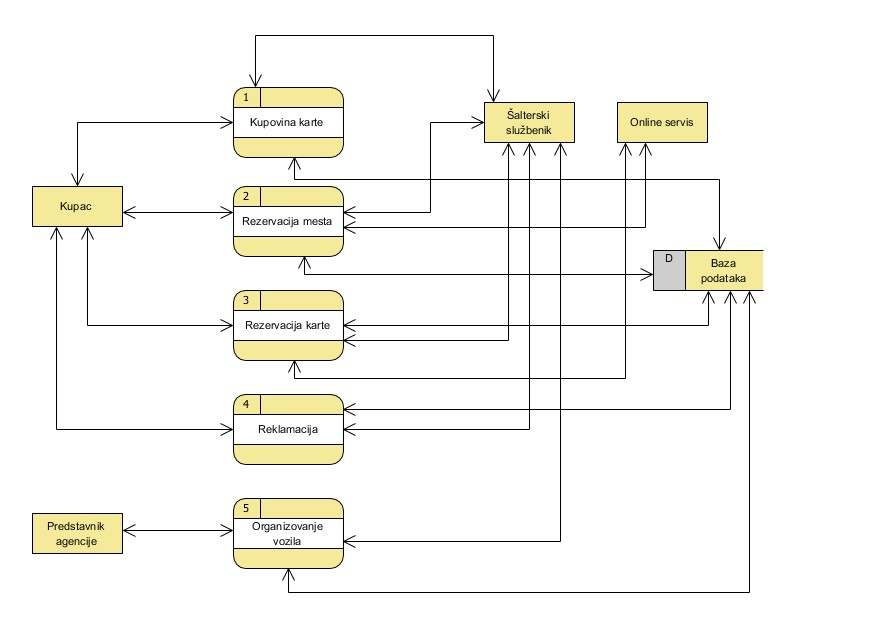
\includegraphics[width=0.7\linewidth]{../Slike/DTP}
	\caption{DTP dijagram nivoa 1}
	\label{fig:dtp}
\end{figure}




\newpage
\section{Akteri}
\subsection{Kupac}
\begin{itemize}
	\item Kupuje kartu
	\item Rezervi\v se kartu
	\item Rezervi\v se mesto
	\item Reklamira kartu
\end{itemize}
\subsection{\v Salterski slu\v zbenik}
\begin{itemize}
	\item Prodaje kartu
	\item Ukoliko je rezervacija ili reklamacija izvr\v sena putem telefona unosi podatke u sistem
\end{itemize}
\subsection{Predstavnik agencije}
\begin{itemize}
	\item Obezbedj{}uje potrebna vozila i voza\v ce
\end{itemize}

\newpage
\section{Slu\v cajevi upotrebe}
\subsection{Online rezervacija karte}
\begin{description}
	\item [$\ast$ Kratak opis: ] Putem veb stranice na\v seg informacionog sistema, kupac mo\v ze dobiti sve potrebne informacije koje se odnose na red vo\v znje, dostupne prevoznike, kao i preciznije detalje o nekoj odredj{}enoj ruti vo\v znje.
	
	\item[$\ast$ U\v cesnici: ] Kupac.
	\item[$\ast$ Preduslovi: ] Pristup internetu.
	\item[$\ast$ Postuslovi: ] Rezervacija karte uspe\v sno poslata u sistem.
	\item[$\ast$ Osnovni tok: ] \ \\
	\renewcommand{\labelenumii}{\Roman{enumii}}
	\begin{enumerate}
		\item Kupac pristupa online sajtu autobuske stanice.
		\item Informi\v se se o dostupnim terminima i redovima vo\v znje za datum i vreme koji mu odgovaraju.
		\item Popunjava formu za rezervaciju karte na kojoj se nalaze detalji poput datuma i vremena polaska.
		\item Sistem vr\v si proveru da li su uneti podaci validni.
		\item Rezervacija karte se pamti u sistem.
		\item Sistem izbacuje poruku kojom obave\v stava kupca o uspe\v snoj ili neuspe\v snoj prijavi.
	\end{enumerate}
	\item[$\ast$ Alternativni tok: ]
	\begin{enumerate}
		\item[4a. ] Ukoliko podaci sa forme za rezervaciju karte nisu korektni sistem odgovaraju\v com porukom obave\v stava kupca i stranica na kojoj se nalazi forma se oslve\v zava
	\end{enumerate}
	
\end{description}
\newpage
\subsection{Online rezervacija mesta}
\begin{description}
	\item [$\ast$ Kratak opis: ] Putem veb stranice na\v seg informacionog sistema, kupac na osnovu postoje\' ce karte(povratne) mo\v ze izvr\v siti rezervaciju mesta za povratak na \v zeljeni datum, u \v zeljeno vreme.
	\item[$\ast$ U\v cesnici: ] Kupac.
	\item[$\ast$ Preduslovi: ] Pristup internetu.
	\item[$\ast$ Postuslovi: ] Rezervacija mesta uspe\v sno poslata u sistem.
	\item[$\ast$ Osnovni tok: ] \ \\
	\renewcommand{\labelenumii}{\Roman{enumii}}
	\begin{enumerate}
		\item Kupac pristupa online sajtu autobuske stanice.
		\item Informi\v se se o dostupnim terminima i redovima vo\v znje za \v zeljeni datum i vreme.
		\item Popunjava formu za rezervaciju mesta, informacije koje su neophodne za rezervaciju mesta kao \v sto su: datum, vreme, prevoznik (ukoliko za zadati datum i vreme imamo vi\v se prevoznika) i broj mobilnog telefona.
		\item Sistem vr\v si proveru da li su uneti podaci validni.
		\item Rezervacija mesta se pamti u sistem.
		\item Sistem izbacuje poruku kojom obave\v stava kupca o uspe\v snoj ili neuspe\v snoj rezervaciji i u slu\v caju uspe\v sne rezervacije \v salje identifikacioni kod na uneti broj mobilnog telefona.
	\end{enumerate}
	\item[$\ast$ Alternativni tok: ]
	\begin{enumerate}
	\item[4a. ] Ukoliko podaci sa forme za rezervaciju karte nisu korektni sistem odgovaraju\' com porukom obave\v stava kupca i stranica na kojoj se nalazi forma se oslve\v zava
	\end{enumerate}
\end{description}
\newpage
\subsection{Rezervacija mesta/karte telefonom}
\begin{description}
	\item [$\ast$ Kratak opis: ] Kupac ima mogu\' cnost da rezervaciju mesta ili karte obavi i putem telefona.
	\item[$\ast$ U\v cesnici: ] Kupac i slu\v zbenik.
	\item[$\ast$ Preduslovi: ]
	\item[$\ast$ Osnovni tok: ] \ \\
	\renewcommand{\labelenumii}{\Roman{enumii}}
	\begin{enumerate}
		\item Kupac poziva broj za rezervacije(mesta/karte).
		\item Slu\v zbenik se javlja i od kupca trazi neophodne informacije: da li je u pitanju rezervacija mesta ili karte, datum polaska i vreme polaska.
		\item U slu\v caju da za iskazani datum i vreme polaska ima vi\v se prevoznika slu\v zbenik naknadno pita kupca kog prevoznika bira.
		\item Kupac bira prevoznika i informacije kompletira brojem telefona.
		\item Sve prethodne podatke slu\v zbenik unosi u sistem.
		\item Sistem vr\v si proveru unetih podataka.
		\item Rezervacija se pamti u sistem.
		\item Sistem izbacuje poruku kojom obave\v stava kupca o uspe\v snoj ili neuspe\v snoj rezervaciji i u slu\v caju uspe\v sne rezervacije \v salje identifikacioni kod na uneti broj mobilnog telefona.		
	\end{enumerate}
	\item[$\ast$ Alternativni tok: ]
	\begin{enumerate}
		\item[6a. ] Ukoliko podaci sa forme za rezervaciju karte nisu korektni sistem odgovaraju\' com porukom obave\v stava kupca i stranica na kojoj se nalazi forma se oslve\v zava.
	\end{enumerate}
\end{description}
\begin{figure}
	\centering
	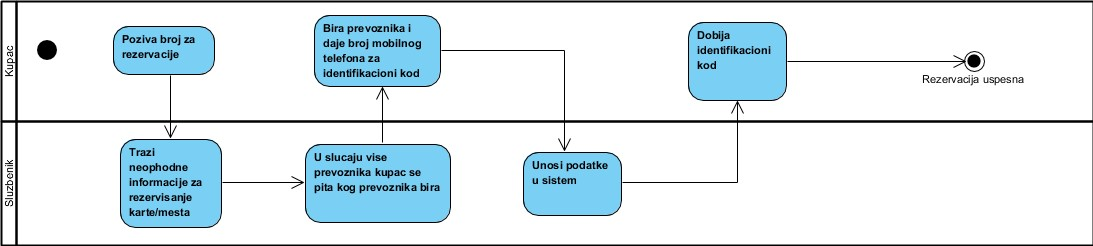
\includegraphics[width=0.7\linewidth]{../Slike/rezervacijaTelefonom}
	\caption{Dijagram aktivnosti - rezervacija telefonom}
	\label{fig:rezervacijatelefonom}
\end{figure}	
\newpage
\subsection{Kupovina karte}
\subsubsection{Kupovina ako karta nije unapred rezervisana}
\begin{description}
	\item[$\ast$ Kratak opis: ] Kupac na \v salteru kupuje kartu za \v zeljenu destinaciju. Slu\v zbenik na \v salteru unosi podatke u sistem i \v stampa kartu ukoliko ima slobodnog mesta u autobusu.
	\item[$\ast$ U\v cesnici: ] Kupac i slu\v zbenik na \v salteru.
	\item[$\ast$ Preduslovi: ] Kupac dolazi na stanicu.
	\item[$\ast$ Tok: ] \ \\
	\begin{enumerate}
		\item Kupac dolazi na \v salter.
		\item Zatra\v zi informacije o vremenima polazaka, prevoznicima i cenama karte ukoliko to vec nije u\v cinio.
		\item Slu\v zbenik na \v salteru mu daje \v zeljene informacije
		\item Kupac se izja\v snjava za vreme polaska i \v zeljenog prevoznika (ukoliko vi\v se prevoznika polazi u isto vreme).
		\item Slu\v zbenik unosi date podatke u sistem.
		\item Sistem proverava da li ima slobodnog mesta u tom terminu.
		\item Ako nema mesta kupovina se smatra neuspe\v snom.
		\item Ina\v ce, slu\v zbenik saop\v stava kupcu da ima slobodnog mesta.
		\item Kupac potvrdjuje da \v zeli da kupi kartu i nagla\v sava da li \v zeli kartu u jednom smeru ili povratnu.
		\item Ukoliko kupac ima pravo na neki od popusta, saop\v stava to slu\v zbeniku i pokazuje odgovaraju\'ca dokumenta kao dokaz.
		\item Slu\v zbenik unosi podatke o popustu i podatke da li je karta povratna ili u jednom smeru.
		\item Sistem \v stampa kartu.
		\item Kupac pla\' ca kartu.
		\item Slu\v zbenik uzima novac i daje kartu kupcu tako da se kupovina smatra uspe\v snom.
	\end{enumerate}
\end{description}

\begin{figure}[!htb] 
	\centering
	\includegraphics[width=1.2\linewidth]{"../Slike/kupovina"}
	\caption{Dijagram aktivnosti - kupovina nerezervisane karte}
	\label{fig:kupovina}
\end{figure}

\subsubsection{Kupovina mesta ako nije unapred rezervisano}
\begin{description}
	\item[$\ast$ Kratak opis: ] Kupac, koji ima povratnu kartu, na \v salteru kupuje mesto za odredjeni termin. Slu\v zbenik na \v salteru unosi podatke u sistem i na karti potvrdjuje mesto i vreme.
	\item[$\ast$ U\v cesnici: ] Kupac i slu\v zbenik na \v salteru.
	\item[$\ast$ Preduslovi: ] Kupac ima povratnu kartu.
	\item[$\ast$ Postuslovi: ] Potvrdjena je kupovina mesta u sistemu.
	\item[$\ast$ Tok: ] \ \\
	\begin{enumerate}
		\item Kupac dolazi na \v salter.
		\item Zatra\v zi informacije o vremenima polazaka za odgovaraju\'ceg prevoznika za odredjeni datum (ako to vec nije ranije u\v cinjeno).
		\item Slu\v zbenik na \v salteru mu daje \v zeljene informacije
		\item Kupac se izja\v snjava za \v zeljeni termin.
		\item Slu\v zbenik unosi odgovaraju\'ce podatke u sistem.
		\item Sistem proverava da li ima slobodnog mesta u datom terminu.
		\item Ako nema mesta kupovina se smatra neuspe\v snom.
		\item Ina\v ce, slu\v zbenik saop\v stava kupcu da ima slobodnog mesta.
		\item Kupac potvrdjuje da li \v zeli da putuje u tom terminu i prila\v ze kartu.
		\item Slu\v zbenik unosi u sistem da kupac \v zeli da putuje.
		\item Sistem mu daje podatak o broju sedi\v sta.
		\item Slu\v zbenik na karti zapisuje broj sedi\v sta, datum i termin putovanja.
		\item Kupac pla\'ca mesto.
		\item Slu\v zbenik uzima novac i vra\'ca kupcu kartu.
	\end{enumerate}
\end{description}

\subsubsection{Kupovina unapred rezervisane karte}
\begin{description}
	\item[$\ast$ Kratak opis: ] Kupac je unapred rezervisao kartu i dolazi na salter da je preuzme.
	\item[$\ast$ U\v cesnici: ] Kupac i slu\v zbenik na \v salteru.
	\item[$\ast$ Preduslovi: ] Kupac je rezervisao kartu za odredjeni termin i odredjenog prevoznika.
	\item[$\ast$ Postuslovi: ] Kupac je dobio papirnu kartu.
	\item[$\ast$ Tok: ] \ \\
	\begin{enumerate}
		\item Kupac dolazi na \v salter.
		\item Saop\v stava slu\v zbeniku da je rezervisao kartu i saop\v stava/pokazuje identifikacioni kod koji je dobio prilikom rezervacije
		\item Slu\v zbenik unosi identifikacioni kod u sistem i tako potvrdjuje kupovinu karte.
		\item Sistem \v cekira da je rezervisana karta preuzeta.
		\item Sistem \v stampa kartu.
		\item Kupac pla\'ca kartu.
		\item Slu\v zbenik uzima novac i daje kartu.
	\end{enumerate}
\end{description}

\subsubsection{Kupovina unapred rezervisanog mesta}
\begin{description}
	\item[$\ast$ Kratak opis: ] Kupac je unapred rezervisao mesto i dolazi na salter da potvrdi.
	\item[$\ast$ U\v cesnici: ] Kupac i slu\v zbenik na \v salteru.
	\item[$\ast$ Preduslovi: ] Kupac ima povratnu kartu i rezervisao je mesto za odredjeni termin kod odgovarajuceg prevoznika.
	\item[$\ast$ Postuslovi: ] Kupac je dobio mesto u autobusu.
	\item[$\ast$ Tok: ] \ \\
	\begin{enumerate}
		\item Kupac dolazi na \v salter.
		\item Saop\v stava slu\v zbeniku da ima rezervisano mesto, saop\v stava/pokazuje identifikacioni kod koji je dobio prilikom rezervacije i prila\v ze kartu
		\item Slu\v zbenik unosi identifikacioni kod u sistem i tako potvrdjuje kupovinu mesta.
		\item Sistem \v cekira da je rezervisano mesto preuzeto.
		\item Slu\v zbenik na karti bele\v zi broj sedi\v sta, vreme i datum putovanja.
		\item Kupac pla\'ca kartu.
		\item Slu\v zbenik uzima novac i vra\'ca kartu kupcu.
	\end{enumerate}
\end{description}

\subsection{Reklamacija}

\begin{description}
  \item[$\ast$ Kratak opis: ] Kupac mo\v ze reklamirati kupljenu kartu na \v salteru. Ukoliko nije prekasno, slu\v zbenik na \v salteru preuzima kartu i osloba\dj a mesto u sistemu i zatim vraca novac korisniku.
  \item[$\ast$ U\v cesnici: ] Kupac i slu\v zbenik na \v salteru
  \item[$\ast$ Preduslovi: ] Kupac ima va\v ze\'cu kartu i do polaska autobusa ima barem sat vremena
  \item[$\ast$ Postuslovi: ] Kupac je vratio kartu i dobio novac natrag
  \item[$\ast$ Osnovni tok: ] \ \\
  \begin{enumerate}
    \item Kupac dolazi na \v salter i obave\v stava slu\v zbenika o nameri da vrati kartu
    \item Slu\v zbenik proverava da li su ispunjeni uslovi za reklamaciju
    \item Ukoliko su uslovi ispunjeni, slu\v zbenik preuzima kartu
    \item Slu\v zbenik poni\v stava kartu i osloba\dj a mesto u sistemu
    \item Slu\v zbenik vra\'ca novac kupcu
  \end{enumerate}
  \item[$\ast$ Alternativni tok]
  \begin{enumerate}
    \item[3a. ]  Ukoliko uslovi nisu ispunjeni, slu\v zbenik obavestava kupca
  \end{enumerate}
  
\end{description}

\subsection{Poni\v stavanje rezervacije karte/mesta - telefonom}
\begin{description}
  \item[$\ast$ Kratak opis: ] Kupac mo\v ze telefonskim putem poni\v stiti rezervaciju karte ili mesta. Ukoliko je rezervacija va\v ze\'ca, slu\v zbenik poni\v stava rezervaciju u sistemu.
  \item[$\ast$ U\v cesnici: ] Kupac i slu\v zbenik
  \item[$\ast$ Preduslovi: ] Kupac ima identifikacioni kod
  \item[$\ast$ Postuslovi: ] Rezervacija je poni\v stena
  \item[$\ast$ Osnovni tok: ] \ \\
  \begin{enumerate}
    \item Kupac zove telefonom i obavestava slu\v zbenika o nameri da poni\v sti
	   rezervaciju karte ili mesta.
    \item Slu\v zbenik trazi identifikacioni kod rezervacije
    \item Kupac daje kod slu\v zbeniku
    \item Sistem proverava da li kod postoji i da li je rezervacija va\v ze\'ca.
    \item Ukoliko su kod i rezervacija va\v ze\'ci, slu\v zbenik poni\v stava 
	   rezervaciju u sistemu
    \item Slu\v zbenik obave\v stava kupca o uspe\v snom poni\v stenju
  \end{enumerate}
  \item[$\ast$ Alternativni tok]
  \begin{enumerate}
    \item[5a. ]  Ukoliko su kod ili rezervacija neva\v ze\'ci, slu\v zbenik obave\v stava kupca o 
		neregularnosti
  \end{enumerate}
  
\end{description}

\subsection{Poni\v stavanje rezervacije karte/mesta - onlajn}
\begin{description}
  \item[$\ast$ Kratak opis: ] Kupac mo\v ze poni\v stiti rezervaciju karte ili mesta putem veb servisa. 
			 	Sistem proverava ispravnost podataka i bri\v se rezervaciju.
  \item[$\ast$ U\v cesnici: ] Kupac
  \item[$\ast$ Preduslovi: ] Kupac ima identifikacioni kod i pristup internetu
  \item[$\ast$ Postuslovi: ] Rezervacija je poni\v stena
  \item[$\ast$ Osnovni tok: ] \ \\
  \begin{enumerate}
    \item Kupac pristupa veb servisu i odabira opciju poni\v stavanja rezervacije.
    \item Servis zahteva identifikacioni kod rezervacije
    \item Kupac unosi kod
    \item Sistem proverava da li kod postoji i da li je rezervacija va\v ze\'ca.
    \item Ukoliko su kod i rezervacija va\v ze\'ci, sistem poni\v stava rezervaciju
    \item Sistem izbacuje poruku kojom obavestava kupca o uspe\v snom poni\v stenju.
  \end{enumerate}
  \item[$\ast$ Alternativni tok]
  \begin{enumerate}
    \item[5a. ]  Ukoliko su kod ili rezervacija neva\v ze\'ci, sistem izbacuje poruku greske kojom obavestava kupca o neregularnosti. 
		neregularnosti
  \end{enumerate}
  
\end{description}

\subsection{Alokacija dodatnih resursa}
\begin{description}
	\item[$\ast$ Kratak opis: ] U slu\v caju da su sva mesta popunjena, sistem obave\v stava predstavnika prevozni\v cke agencije da je potrebno jo\v s resursa. 
	\item[$\ast$ U\v cesnici: ] Predstavnik agencije.
	\item[$\ast$ Preduslovi: ] Nema vi\v se mesta u trenutno rasporedjenim autobusima.
	\item[$\ast$ Postuslovi: ] Povratna informacija da li prevoznik ima odgovaraju\'ce raspolo\v zive resurse.
	\item[$\ast$ Tok: ] \ \\
	\begin{enumerate}
		\item Sistem obave\v stava predstavnika prevozni\v cke agencije da su potrebni dodatni resursi.
		\item Predstavnik agencije mu \v salje odgovor da li mo\v ze da zameni teku\'ce vozilo vozilom ve\'ceg kapaciteta ili da uvede dodatno.
		\item Ukoliko postoje odgovaraju\'ci resursi, bele\v ze se podaci o njima u sistem.
	\end{enumerate}
\end{description}

\newpage

\section{Baza podataka}
\subsection{Model baze podataka}
\begin{figure}[h]
	\centering
	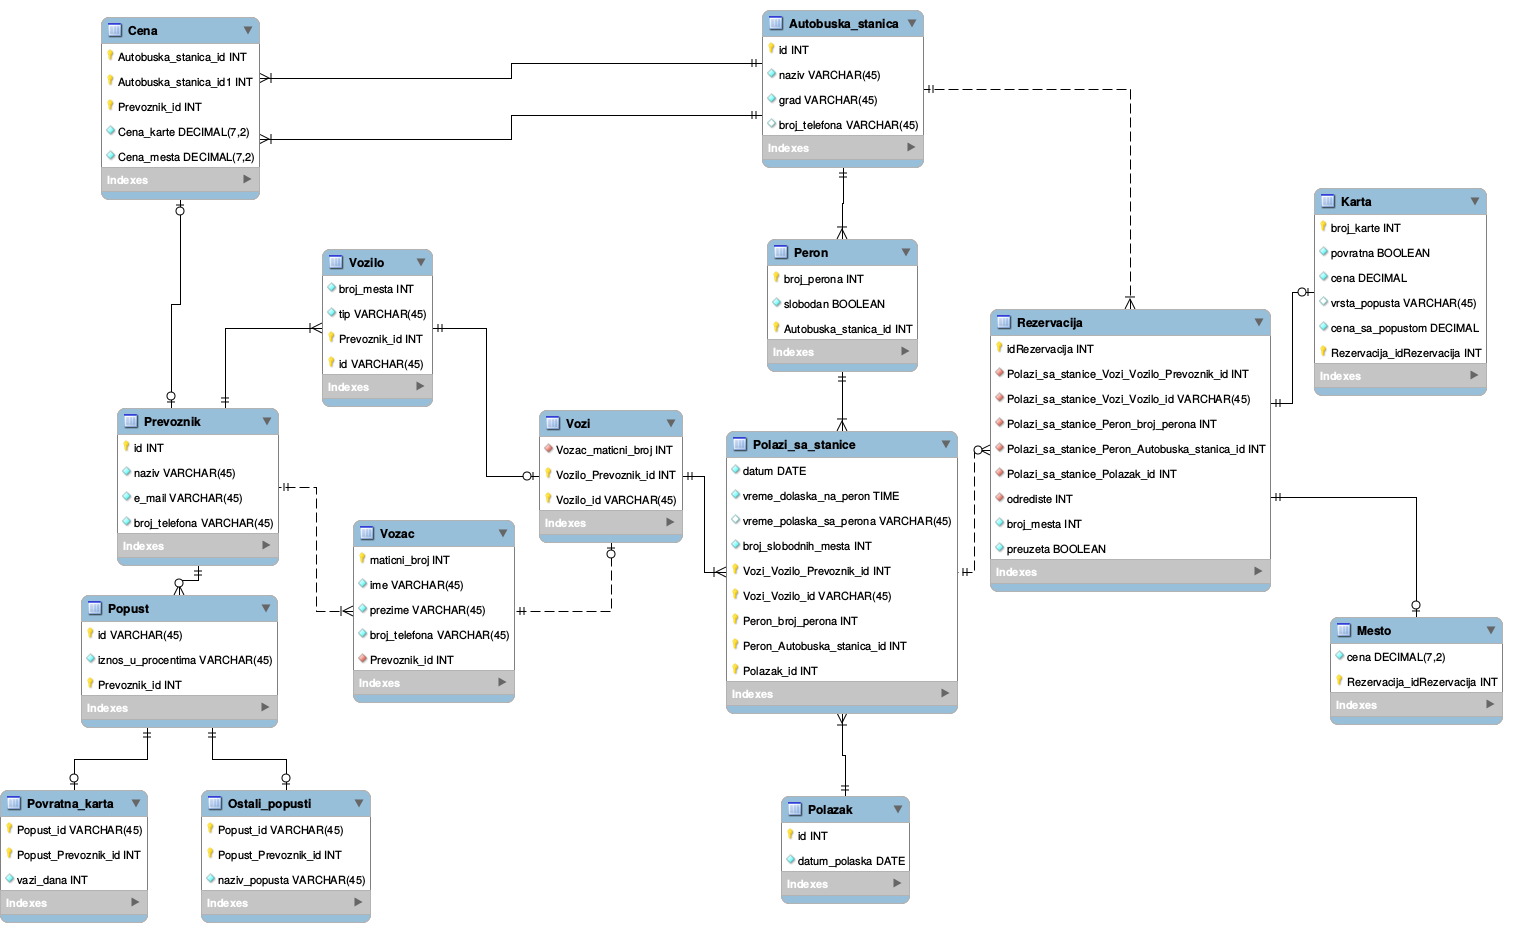
\includegraphics[width=17cm, height = 12.5cm]{../Slike/baza.png}
	\caption{Model baze podataka}
	\label{fig:baza}
\end{figure}	
\subsection{Opis entiteta}

\textbf{Autobuska\_stanica} \\
Opisuje odredjenu autobusku stanicu.
\begin{itemize}
	\item id
	\item naziv
	\item grad
	\item broj\_telefona
\end{itemize}
\textbf{Peron} \\
Svaka stanica ima bar jedan peron.
\begin{itemize}
	\item broj\_perona
	\item slobodan
	\item Autobuska\_stanica\_id 
\end{itemize}
\textbf{Polazak} \\
\begin{itemize}
	\item id
	\item datum\_polaska
\end{itemize}
\textbf{Prevoznik} \\
\v Cuva podatke o prevozniku.
\begin{itemize}
	\item id
	\item naziv
	\item e\_mail
	\item broj\_telefona
\end{itemize}
\textbf{Vozac} \\
Sadr\v zi informacije o voza\v cima.
\begin{itemize}
	\item maticni\_broj
	\item ime
	\item prezime
	\item broj\_telefona
	\item Prevoznik\_id
\end{itemize}
\textbf{Vozilo} \\
Informacije o vozilima koje obezbedjuje odredjeni prevoznik.
\begin{itemize}
	\item id
	\item Prevoznik\_id
	\item broj\_mesta
	\item tip
\end{itemize}
\textbf{Vozi} \\
Veza izmeju vozila i voza\v ca.
\begin{itemize}
	\item Vozac\_maticni\_broj
	\item Vozilo\_Prevoznik\_id
	\item Vozilo\_id
\end{itemize}
\textbf{Polazi\_sa\_stanice} \\
Podaci o vremenu kada koji autobus kre\'ce sa kod perona i stanice.
\begin{itemize}
	\item datum
	\item vreme\_dolaska\_na\_peron
	\item vreme\_polaska\_sa\_perona
	\item broj\_slobodnih\_mesta
	\item Vozi\_Vozilo\_Prevoznik\_id
	\item Vozi\_Vozilo\_id
	\item Peron\_broj\_perona
	\item Peron\_Autobuska\_stanica\_id
	\item Polazak\_id
\end{itemize}
\textbf{Rezervacija}\\
Informacije o rezervaciji karte ili mesta.
\begin{itemize}
	\item idRezervacija
	\item Polazi\_sa\_stanice\_Vozi\_Vozilo\_Prevoznik
	\item Polazi\_sa\_stanice\_Vozi\_Vozilo\_id
	\item Polazi\_sa\_stanice\_Peron\_broj\_perona
	\item Polazi\_sa\_stanice\_Peron\_Autobuska\_stanica
	\item Polazi\_sa\_stanice\_Polazak\_id
	\item odrediste - id odredi\v sne stanice
	\item broj\_mesta
	\item preuzeta
\end{itemize}
\textbf{Karta}
\begin{itemize}
	\item broj\_karte
	\item Rezervacija\_idRezervacija
	\item povratna
	\item cena
	\item vrsta\_popusta
	\item cena
	\item cena\_sa\_popustom
\end{itemize}
\textbf{Mesto}
\begin{itemize}
	\item cena
	\item Rezervacija\_idRezervacija
\end{itemize}
\textbf{Popust} \\
Sadr\v zi podatke o popustima koje daje odredjeni prevoznik.
\begin{itemize}
	\item id
	\item iznos\_u\_procentima
	\item Prevoznik\_id
\end{itemize}
\textbf{Povratna\_karta}\\
Informacije o popustu na povratnu kartu.
\begin{itemize}
	\item Popust\_id
	\item Popust\_Prevoznik\_id
	\item vazi\_dana
\end{itemize}
\textbf{Ostali\_popusti} \\
Pored popusta za povratnu kartu, prevoznici daju popust i za odredjene kategorije gradjana.
\begin{itemize}
	\item Popust\_id
	\item Popust\_Prevoznik\_id
	\item naziv\_popusta
\end{itemize}
\textbf{Cena}\\
Informacije o cenama izmedju dve stanice za odredjenog prevoznika.
\begin{itemize}
	\item Autobuska\_stanica\_id
	\item Autobuska\_stanica\_id1
	\item Prevoznik\_id
	\item cena\_karte
	\item cena\_mesta
\end{itemize}
\textbf{Zaposleni}
Informacije o zaposlenima na odredjenoj stanici.
\begin{itemize}
	\item id
	\item korisnicko\_ime
	\item sifra
	\item Ime
	\item Prezime
	\item broj\_telefona
	\item Autobuska\_stanica\_id
\end{itemize}
\newpage
\section{Arhitektura}
\subsection{Uvod}
Karakteristike arhitekture informacionog sistema za medjugradski autobuski saobra\' caj.

\begin{description}
	\item[$\ast$ Tip aplikacije:] Web aplikacija - i za klijente i za slu\v zbenike.
	\item[$\ast$ Strategija isporu\v civanja:] Jedan serverski i vi\v se klijentskih ra\v cunara.
	\item[$\ast$ Tehnologije:] HTML5, CSS, JS, PHP, MySql.
	\item[$\ast$ Prate\' ce komponente:] \ \\
		\begin{enumerate}
			\item Logovanje na sistem:
				\begin{enumerate}
					\item[$\bullet$] Podsistem za logovanje slu\v zbenika
						\begin{enumerate}
							\item[$\cdot$] Komponenta za validaciju podataka
							\item[$\cdot$] GUI komponenta za u\v citavanje podataka o korisni\v ckom imenu i lozinci
						\end{enumerate}
					\item[$\bullet$] Podsistem za logovanje kupca
					\begin{enumerate}
						\item[$\cdot$] Komponenta za validaciju podataka
						\item[$\cdot$] GUI za u\v citavanje broja telefona i identifikacionog koda
					\end{enumerate}
					
				\end{enumerate}
			\item Backup baze - podsistem koji pravi kopiju baze
				\begin{enumerate}
					\item[$\bullet$] Schedule backup - na mese\v cnom ili nedeljnom nivou
					\item[$\bullet$] On-demand backup
				\end{enumerate}
			\item Podr\v ska: dokumentacija, kontakt, podrska
		\end{enumerate}
	\item[$\ast$ Tip arhitekture:] Klijent - server arhitektura
	\item[$\ast$ 4 sloja:] prezentacioni sloj, klijent kontroler, server kontroler, sloj podataka. 
	\item[$\ast$] Klijent kontroler izvr\v sava validaciju podataka i autentifikaciju/autorizaciju, a server kontroler predstavlja serversku obradu podataka. Prezentacioni sloj pru\v za interfejs preko koga klijent mo\v ze i\v zvr\v siti rezervaciju karte/mesta ili reklamaciju istog, dok u slu\v caju slu\v zbenika pokre\' ce mehanizme za logovanje na sistem, a zatim pru\v za mogu\' cnost za unos podataka o kupovini karte/mesta i unos podataka o rezervacijama koje su obavljene telefonom.
\end{description}

\begin{figure}[!htb] 
	\centering
	\includegraphics[width=1.2\linewidth]{"../Slike/arhitektura"}
	\caption{Arhitektura sistema}
	\label{fig:arhitektura}
\end{figure}

\iffalse
\subsection{Alokacija dodatnih resursa}
\begin{description}
	\item[$\ast$ Kratak opis: ] U slu\v caju da su sva mesta popunjena, sistem obave\v stava predstavnika prevozni\v cke agencije da je potrebno jo\v s resursa. 
	\item[$\ast$ U\v cesnici: ] Predstavnik agencije.
	\item[$\ast$ Preduslovi: ] Nema vi\v se mesta u trenutno rasporedjenim autobusima.
	\item[$\ast$ Postuslovi: ] Povratna informacija da li prevoznik ima odgovaraju\'ce raspolo\v zive resurse.
	\item[$\ast$ Tok: ] \ \\
	\begin{enumerate}
		\item Sistem obave\v stava predstavnika prevozni\v cke agencije da su potrebni dodatni resursi.
		\item Predstavnik agencije mu \v salje odgovor da li mo\v ze da zameni teku\'ce vozilo vozilom ve\'ceg kapaciteta ili da uvede dodatno.
		\item Ukoliko postoje odgovaraju\'ci resursi, bele\v ze se podaci o njima u sistem.
	\end{enumerate}
\end{description}
\fi
